\documentclass[
    11pt,
    a4paper,
    sfdefaults=false,
    toc=chapterentrywithdots,
    oneside, % or twoside for printing
    openany, % or openright for printing
    titlepage,
    parskip=half,
    headings=normal,  % reduces heading size
    listof=totoc,
    bibliography=totoc,
    index=totoc,
    captions=tableheading,  % caption below table
    chapterprefix,
    listof=flat,
    numbers=noendperiod, % for omitting the trailing dot after chapter and section numbers
    final
]{scrbook}

% !TeX spellcheck = de_DE 

% details about your thesis
\newcommand{\titel}{Fehlertoleranz mit Reed-Solomon}
\newcommand{\artderarbeit}{Schriftlicher Bericht}  % {Bachelorarbeit,Masterarbeit}
\newcommand{\autor}{Jonas Lang}
\newcommand{\studiengang}{Informatik}
\newcommand{\matrikelnr}{363\,0314}
\newcommand{\erstgutachter}{Prof.\,Dr.~Korbinian Riedhammer}
\newcommand{\zweitgutachter}{Prof.\,Dr.~Bartosz von\,Rymon\,Lipinski}
\newcommand{\betreuer}{Prof.\,Dr.~Axel Hein}
\newcommand{\unternehmen}{Musterfirma GmbH}
\newcommand{\logo}{figures/TH-Nuernberg-RGB.png}
\newcommand{\keywords}{error correction, reed solomon, encoding, decoding}
\newcommand{\submissionDate}{25. Juni 2024}

% custom head and foot
\usepackage[automark]{scrlayer-scrpage}
\pagestyle{scrheadings}
\ihead{\headmark}
\chead{}
%\ohead{\pagemark}

\RedeclareSectionCommand[tocindent=0pt]{section}
\RedeclareSectionCommand[tocindent=0pt]{subsection}
%\RedeclareSectionCommand[tocnumwidth=70pt]{chapter}

\usepackage{scrhack}

% Bibliography
\usepackage[style=ieee, backend=biber, dashed=false]{biblatex}
\addbibresource{refs.bib}
\AtEveryBibitem{\clearfield{language}}
\setcounter{biburllcpenalty}{7000}
\setcounter{biburlucpenalty}{8000}
% to force "et al." instead of "u.a.":
\DefineBibliographyStrings{german}{
	andothers = {{et\,al\adddot}},
}

% other packages
\usepackage[utf8]{inputenc}
\usepackage[T1]{fontenc}
\usepackage{lmodern,relsize,textcomp,csquotes}
\usepackage{amsmath,amsfonts} % math formulas
\usepackage[english, ngerman]{babel}  % flip for German thesis
\usepackage[final]{graphicx}
\usepackage{setspace,geometry,xcolor}
\usepackage{makeidx}
\usepackage{paralist,ifthen,todonotes}
\usepackage{url}
\usepackage[toc]{glossaries}
\usepackage{pdfpages}
\usepackage{enumitem} % for list and enumerations

% table setup
\usepackage{longtable}
\usepackage{array}
\usepackage{ragged2e}
\usepackage{lscape}
\usepackage{booktabs} % for advanced tables

% pdf hyperref
\usepackage[
    bookmarks=true,
    bookmarksopen=true,
    bookmarksnumbered=true,
    bookmarksopenlevel=1,
    pdftitle={\titel},
    pdfauthor={\autor},
    pdfcreator={\autor},
    pdfsubject={\titel},
    pdfkeywords={\keywords},
    pdfpagelabels=true,
    hidelinks,
    colorlinks=false,
    linkcolor=red,
    urlcolor=magenta,
    anchorcolor=black,
    citecolor=cyan,
    filecolor=magenta,
    menucolor=red,
    plainpages=false,
    hypertexnames=true,
    linktocpage=true,
]{hyperref}

% configure your listings style
\usepackage{listings}
\lstset{
	tabsize=3,
	extendedchars=true,
	frame=single,
	showstringspaces=true,
	numbers=left,
	numberstyle=\small,
	breakautoindent=true
}

% page setup
% \setlength{\topskip}{\ht\strutbox}
\geometry{paper=a4paper,left=2.5cm,top=3.0cm,} % bindingoffset=.8cm for printing
\onehalfspacing
\frenchspacing
\clubpenalty = 10000
\widowpenalty = 10000 
\displaywidowpenalty = 10000

% some commands
\newcommand{\ua}{\mbox{u.\,a.\ }}
\newcommand{\zB}{\mbox{z.\,B.\ }}
\newcommand{\dahe}{\mbox{d.\,h.,\ }}
\newcommand{\bzw}{\mbox{bzw.\ }}
\newcommand{\bzgl}{\mbox{bzgl.\ }}
\newcommand{\eg}{\mbox{e.\,g.\ }}
\newcommand{\ie}{\mbox{i.\,e.\ }}
\newcommand{\wrt}{\mbox{w.\,r.\,t.\ }}
\newcommand{\etal}{\mbox{\emph{et\,al.\ }}}

% load glossary 
\loadglsentries{glossary}
\makenoidxglossaries

\begin{document}

\setcounter{secnumdepth}{3}  % numerate subsections
\setcounter{tocdepth}{2}  % ...but don't include them in toc

\frontmatter
\thispagestyle{empty}
\pdfbookmark[1]{Cover}{cov}
\begin{titlepage}

\begin{center}

\includegraphics[width=\linewidth]{figures/ohm-logo.png}\\[1cm]
\LARGE{Fakultät Informatik}\\[2cm]

\huge
\textbf{\titel}\\[1cm]
%
\Large
\artderarbeit~im Fach \\ \course\\[1cm]
%
\large
vorgelegt von

\Large
\autor\\
\small
Matrikelnummer \matrikelnr\\[0.5cm]
\normalsize
am \submissionDate\\

\vspace*{\fill}

\large
\begin{tabular}{p{3cm}p{8cm}}\\
%discomment "Betreuer" and "Unternehmen" for a thesis in a company
%Betreuer: & \quad \betreuer\\
%Unternehmen: & \quad \unternehmen
\end{tabular}
\end{center}

\begin{center}
\copyright\,\the\year
\end{center}

\vspace{-0.5cm}
\singlespacing
\small
\noindent Dieses Werk einschließlich seiner Teile ist \textbf{urheberrechtlich geschützt}.
Jede Verwertung außerhalb der engen Grenzen des Urheberrechtsgesetzes ist ohne Zustimmung des Autors unzulässig und strafbar.
Das gilt insbesondere für Vervielfältigungen, Übersetzungen, Mikroverfilmungen sowie die Einspeicherung und Verarbeitung in elektronischen Systemen.

\end{titlepage}
\cleardoublepage

% download the following form (requires VPN) and complete it (hit save in your editor)
% https://intern.ohmportal.de/fileadmin/Public_Docs/SB/SB_0009_FO_Pruefungsrechtliche_Erklaerung_und_Erklaerung_zur_Veroeffentlichung_der_Abschlussarbeit_public.pdf
%\includepdf{SB_0009_FO_Pruefungsrechtliche_Erklaerung_und_Erklaerung_zur_Veroeffentlichung_der_Abschlussarbeit_public.pdf}\cleardoublepage

\thispagestyle{empty}
\section*{Kurzdarstellung}
\label{sec:kurzdarstellung}
Kurze Zusammenfassung der Arbeit, höchstens halbe Seite.
Deutsche Fassung auch nötig, wenn die Arbeit auf Englisch angefertigt wird.


\section*{Abstract}
\label{sec:abstract}
\emph{Only if thesis is written in English.}
\cleardoublepage

\tableofcontents

\listoffigures
\cleardoublepage

\listoftables
\cleardoublepage

\mainmatter
\chapter{Einleitung}\label{ch:intro}

\section{Motivation}\label{sec:motivation}

In der heutigen digitalen Welt ist die Zuverlässigkeit und Integrität von Daten von zentraler Bedeutung. 
Täglich werden riesige Mengen an Informationen über verschiedene Kommunikationskanäle übertragen und auf unterschiedlichsten Medien gespeichert. 
Dabei ist es unvermeidlich, dass einige Daten durch Rauschen, physische Beschädigungen oder andere Störfaktoren verfälscht werden. 
Die Gewährleistung der Genauigkeit und Verfügbarkeit von Informationen ist insbesondere in Bereichen der Telekommunikation, Datenarchivierung und digitalen Medien von entscheidender Bedeutung. 
Die Sicherstellung dieser Faktoren stellt jedoch eine ernsthafte Herausforderung dar. 
Fehlererkennungs- und -korrekturverfahren sind daher unverzichtbare Werkzeuge, um die Qualität und Zuverlässigkeit der übermittelten oder gespeicherten Daten sicherzustellen \cite{petersonErrorcorrectingCodes1972}.

Um das zu erreichen, werden bei der Kanalcodierung die zu speichernden oder zu übertragenden Daten beim Encodierungsprozess mit Redundanz, also zusätzlichen Informationen, die zur Fehlererkennung und -korrektur dienen, angereichert. 
Im Decodierungsprozess wird an Hand der Redundanz überprüft, ob Fehler aufgetreten sind und ob diese korrigiert werden können. 
Dadurch kann die Integrität der empfangenen Daten bewertet werden.

Eine besonders effektive Methode zur Fehlerkorrektur sind die Reed-Solomon-Codes, also das ursprüngliche Verfahren und alle Weiterentwicklungen.
Die ursprüngliche Version wurde 1960 von den Mathematikern Irving S. Reed und Gustave Solomon entwickelt \cite{reedPolynomialCodesCertain1960}. 
Reed-Solomon-Codes zeichnen sich durch ihre Fähigkeit aus, so viele Fehler wie die Anzahl der hinzugefügten redundanten Informationen zu erkennen und sogar die Hälfte dieser zu korrigieren.
In dieser Arbeit liegt der Fokus auf der Fehlerkorrektur.

\section{Zielsetzung der Arbeit}\label{sec:objective}

Obwohl diese Codes in vielen alltäglichen Technologien wie CDs oder QR-Codes weit verbreitet sind, ist die zugrundeliegende Mathematik und konkrete Implementierung eher unbekannt \cite{wickerReedSolomonCodes1994}. 
Ziel dieser Arbeit ist es, die Reed-Solomon-Codes vorzustellen und deren Funktionsweise zu erklären. 
Dazu wird nach einer kurzen historischen Betrachtung die der Kanalcodierung zu Grunde liegenden Mathematik beschrieben.
Anschließend wird die Funktionsweise des ursprünglichen Ansatzes der beiden Mathematikern und eine Weiterentwicklung, der Berlekamp-Welch-Algorithmus, erläutert.
Des Weiteren wird beleuchtet, wie diese Verfahren in der Praxis Anwendung finden. 

\chapter{Entwicklung}\label{ch:development}

Die Reed-Solomon-Codes wurden 1960 von den amerikanischen Mathematikern Irving S. Reed und Gustave Solomon am Licoln Laboratory des MIT entwickelt.
Sie veröffentlicheten das Paper \textquote{Polynomial codes over certain finite fields}, indem das neu entworfene Fehlerkorrekturverfahren beschrieben wird.
Dabei handelt es sich um Vorwärtskorrektur-Verfahren, welches eigenständig Fehler erkennen und beseitigen kann \cite{wickerReedSolomonCodes1994}.
Durch diese Veröffentlichung wurde eine neue Klasse von \acrlong{ecc}s (\acrshort{ecc}) geschaffen. 
Sie gehört zu der Gruppe der linearen, zyklischen Block-Codes, \dahe zu codierende Daten werden in Wörter der Länge \(n\) geteilt und einzeln weiterverarbeitet \cite{friedrichsKanalcodierung1996}. Ein Ausschnitt der Code-Hierarchie ist in Abbildung \ref{fig:eccHierarchy} dargestellt.

\begin{figure}[h]
	\centering
	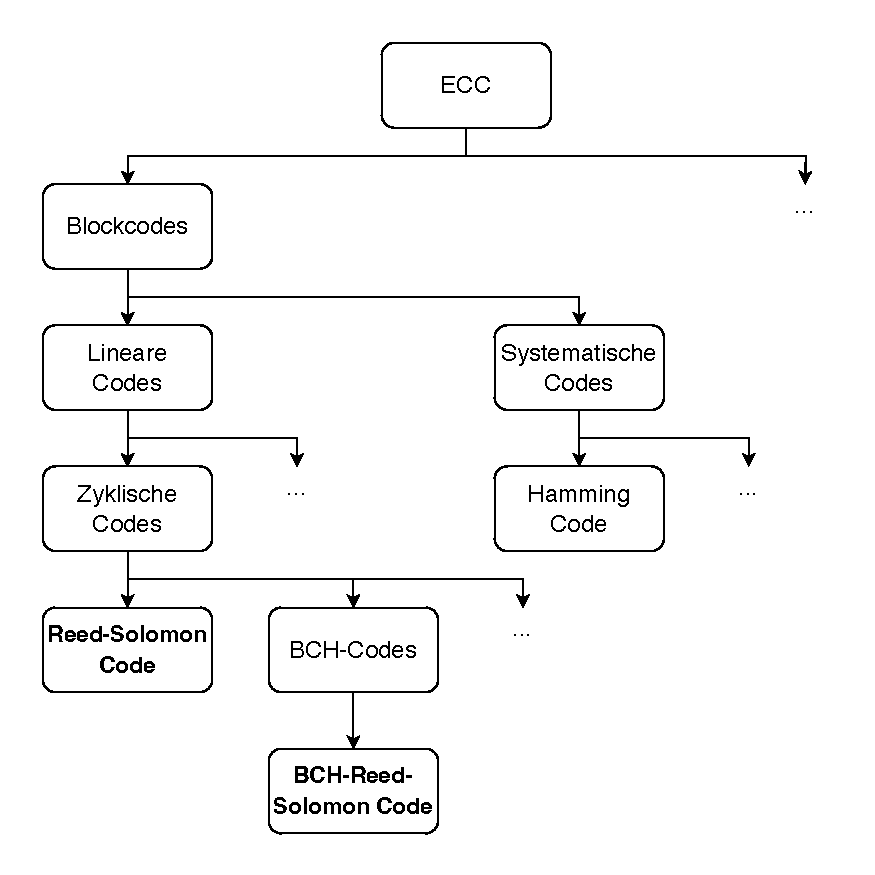
\includegraphics[width=0.9\textwidth]{figures/Codeklassen.drawio.pdf}
	\caption{Ausschnitt der Hierarchie von \acrshort{ecc}}
	\label{fig:eccHierarchy}
\end{figure}

Allerdings war für das Reed-Solomon Verfahren anfangs noch kein effizienter Decodieralgorithmus bekannt, weshalb daran weiter geforscht und weiterentwickelt wurde.
1963 stellte J. J. Stone ein Reed-Solomon-Code vor, der auf dem Schema der auf dem \acrfull{bch} Verfahren basiert \cite{petersonErrorcorrectingCodes1972}.
Dieser Ansatz wird zwar auch als Reed-Solomon-Code bezeichnet, es handelt sich dabei aber um ein weiteres Verfahren, welches seperat vom ursprünglichen Ansatz weiterentwickelt wurde.
Nachdem für die \acrshort{bch}-Codes 1969 ein effizienter Algorithmus, der so genannte Berlekamp-Massey Algorithmus, gefunden wurde, war auch der Einsatz der auf \acrshort{bch} basierende Reed-Solomon-Code in der Praxis verwendbar \cite{berlekampNonbinaryBCHDecoding1968, masseyShiftregisterSynthesisBCH1969}.

Dieses Verfahrens fand zum ersten Mal Anwendung im Jahr 1977 beim Voyager Programm der NASA \cite{wickerReedSolomonCodes1994}. 
Dadurch konnte eine robustere Kommunikation zwischen dem Raumfahrzeug und dem Raumfahrtkontrollzentrum bei einer großen Entfernung zur Erde gewährleistet werden \cite{ludwigVoyagerTelecommunications2002}.
Das erste kommerzielle, an den Endkunden gerichtete Produkt, in dem das Reed-Solomon Verfahren anwendung fand, war 1982 die \acrfull{cd}.

Im Jahr 1986 ermöglichte der Berlekamp-Welch-Algorithmus eine entscheidende Weiterentwicklung. Entwickelt von Elwyn Berlekamp und Lloyd Welch, verbesserte dieser Algorithmus die Effizienz des ursprünglichen Reed-Solomon-Schemas erheblich. Diese Weiterentwicklung förderte die Verbreitung der Reed-Solomon-Codes in verschiedenen Anwendungsbereichen. Eine detailiierte beschreibeung dieser findet sich in Kapitel \ref{ch:application}.

Die kontinuierliche Weiterentwicklung und Anwendung der Reed-Solomon-Codes in verschiedenen Bereichen zeigt die Bedeutung und Vielseitigkeit dieser Fehlerkorrekturverfahren. Um ein tieferes Verständnis der Funktionsweise und der mathematischen Prinzipien hinter diesen Codes zu erlangen, ist es unerlässlich, die theoretischen Grundlagen zu betrachten. Im nächsten Kapitel werden daher die mathematischen Konzepte und Algorithmen erläutert, die den Reed-Solomon-Codes zugrunde liegen.
\chapter{Theoretische Grundlagen}\label{ch:foundation}

In this chapter, we're actually using some code!

\begin{lstlisting}[language=Python,caption={This is an example of inline listing},captionpos=b]
x = 1
if x == 1:
    # indented four spaces
    print("x is 1.")

\end{lstlisting}

You can also include listings from a file directly:

\lstinputlisting[language=Python,caption={This is an example of included listing},captionpos=b]{listings/example.py}

\chapter{Experiments}\label{ch:experiments}


\chapter{Anwendungen}\label{ch:application}

Reed-Solomon-Codes haben sich als äußerst vielseitig und effektiv in einer Vielzahl von Anwendungen erwiesen, insbesondere in Bereichen, die eine hohe Zuverlässigkeit und Robustheit bei der Datenübertragung und -speicherung erfordern \cite{WasIstReedSolomonVerfahren2022}. 
Im Folgenden werden einige der wichtigsten Anwendungsgebiete dieses Fehlerkorrekturverfahren beschrieben.
Die konkreten Umsetzungsparameter finden sich im Anhang \ref{app:parameter} auf Seite \pageref{app:parameter}, sofern sie verfügbar sind.

\section{Satelliten- und Weltraumkommunikation}

Eine der frühesten Anwendungen der Reed-Solomon-Codes war im Bereich der Satelliten- und Weltraumkommunikation. 
Ein bemerkenswertes Beispiel ist das Voyager-Programm der \mbox{NASA}. Seit 1977 werden Reed-Solomon-Codes verwendet, um die Kommunikation zwischen den Voyager-Raumfahrzeugen und der Erde zu sichern. 
Andere Projekte mit Reed-Solomon-Codes im Einsatz sind zum Beispiel der \textit{Mars Pathfinder} und die Raumsonde \textit{Galileo} \cite{wickerReedSolomonCodes1994}.

Die enorme Entfernung der Raumfahrzeuge zur Erde stellt eine besondere Herausforderung an die Datenintegrität. 
Durch kosmische Strahlung und andere Störeinflüsse werden Übertragungsfehlern verursacht, die Reed-Solomon-Codes korrigieren können und  so zur erfolgreichen Übermittlung von wissenschaftlichen Daten über große Distanzen beitragen \cite{ludwigVoyagerTelecommunications2002}.

\section{Broadcasting und digitale Fernsehtechnik}

Im Bereich des Broadcasting, insbesondere bei der digitalen Fernsehtechnik, spielen Reed-Solomon-Codes eine entscheidende Rolle. 
Sie werden verwendet, um die Qualität und Zuverlässigkeit von digitalen TV-Signalen zu verbessern. 
Durch die Implementierung von Reed-Solomon-Codes können Übertragungsfehler, die durch atmosphärische Störungen oder andere Übertragungsprobleme entstehen, effektiv korrigiert werden, was zu einer stabileren und hochwertigeren Signalübertragung führt.
Genutzt wird das Reed-Solomon-Verfahren beispielsweise von dem amerikanischen Standard \acrfull{atsc} und dem europäischen Pendant \acrfull{dvb} \cite{ilievAnalysisEvaluationReedSolomon2008}.
DVB beinhaltet verschiedene Standards, welche mittlerweile andere Verfahren, wie zum Beispiel \acrshort{bch}-Codes verwenden. 
Beispielhaft für ein auf Reed-Solomon basierendes Protokoll ist \acrshort{dvb-h} \cite{DVBH2024}. 

\section{Speichergeräte und optische Datenträger}

Reed-Solomon-Codes sind bei der Sicherstellung der Datenintegrität beim Speichern von Daten essentiell. 
Bei optischen Datenträgern, die seit der Einführung der \acrfull{cd} im Jahr 1982 weit verbreitet sind, werden Reed-Solomon-Codes zur Fehlerkorrektur bei der Speicherung und Wiedergabe von digitalen Audio- und Videodaten verwendet. Dazu zählen neben den \acrshort{cd} auch die \acrfull{dvd} und die Blu-Ray-Disc. 
Diese Codes können Fehler erkennen und korrigieren, die durch Kratzer, Staub oder andere physische Beschädigungen an den Discs verursacht werden \cite{changReedSolomonProductCodeRSPC1998}. 

In \acrshort{raid}-Systemen (\acrlong{raid}), zum Beispiel verwendet für die Aufbewahrung von Backups, ermöglichen sie die Korrektur von Fehlern, wodurch ein Ausfall eines physischen Laufwerks nicht zum Verlust der auf dem System gespeicherten Daten führt.
Diese \acrshort{raid}-Systeme bieten verschiedene Modi zur redundanten Datenspeicherung.
Eine davon ist RAID6, welches auf Reed-Solomon-Codes basiert \cite{RAIDStorageTechnology2021}.

\section{Datenübertragung und digitale Kommunikation}

Reed-Solomon-Codes finden auch breite Anwendung in der digitalen Kommunikation, einschließlich der Datenübertragung über das Internet und in Mobilfunknetzen. 
Sie werden eingesetzt, um die Integrität von Datenpaketen zu gewährleisten, die über potenziell fehleranfällige Kanäle übertragen werden. 
Reed-Solomon-Codes verwendende Standards sind z.B. \acrshort{wimax} und \acrshort{dsl}.
Allerdings ist die genaue Umsetzung dieser Protokolle nicht öffentlich \cite{vermillionEndtoEndDSLArchitectures2003}.

\section{Zweidimensionale Barcodes}

Reed-Solomon-Codes sind auch in der Optoelektronik weit verbreitet. Beispiele hierfür sind MaxiCode, Datamatrix, AztecCode und QR-Code. 
Diese Codes nutzen die Fehlerkorrekturfähigkeiten von Reed-Solomon, um sicherzustellen, dass die gespeicherten Informationen auch dann korrekt ausgelesen werden können, wenn Teile des Codes beschädigt oder verdeckt sind. 
Dies ist besonders wichtig in Anwendungen, bei denen die Zuverlässigkeit der Datenlesung entscheidend ist, wie z.B. in der Logistik, im Einzelhandel und in Fragen der Sicherheit \cite{tiwariIntroductionQRCode2016}.
Bei QR-Codes gibt es verschiedenen Varianten von \textquote{Low} bis \textquote{High}, welche unterschiedlich viel Fehlertoleranz besitzen \cite{QRCode2024}.
Wie QR-Codes diese Fehlertoleranz umsetzten, ist ausführlich in Anhang \ref{app:qr-code} auf Seite \pageref{app:qr-code} beschrieben.
\chapter{Fazit und Ausblick}\label{ch:summary}

\section{Aktuelle Entwicklungen}

Reed-Solomon-Codes bleiben auch heute eine relevante Technologie in der Fehlerkorrektur und -detektion, obwohl sie in den letzten Jahrzehnten aus Kostengründen durch neue Methoden ergänzt und teilweise ersetzt wurden \cite{ilievAnalysisEvaluationReedSolomon2008}. 

Allerdings wird die Integration von Reed-Solomon-Codes in modernen Kom"-mu"-ni"-kations- und Speichertechnologien immer bedeutender.
Insbesondere im Bereich der drahtlosen Kommunikation und der Netzwerkcodierung werden Reed-Solomon-Codes in Kombination mit anderen Fehlerkorrekturmethoden eingesetzt, um eine höhere Zuverlässigkeit zu gewährleisten \cite{conOptimalTwoDimensionalReed2024}.

\section{Zukünftige Perspektiven}

In der Zukunft werden Reed-Solomon-Codes weiterhin eine wichtige Rolle in der Datenübertragung und -speicherung spielen, insbesondere in Kombination mit anderen Technologien. 
Die Entwicklungen im Bereich der Quantenkommunikation und Quantencomputing bieten neue Möglichkeiten, in denen klassische Fehlerkorrekturverfahren wie Reed-Solomon-Codes integriert werden könnten, um Systeme zu schaffen, die auch Quanteninformationen fehlertoleranter machen \cite{grasslQuantumReedSolomonCodes1999}.

Darüber hinaus wird die steigende Nachfrage nach robusten und zuverlässigen Speichersystemen in Bereichen wie Cloud-Computing und Big Data voraussichtlich die Weiterentwicklung und Anwendung von Reed-Solomon-Codes beeinflussen. 
Die zunehmende Komplexität und Größe von Datensätzen erfordert fortschrittliche Fehlerkorrekturmechanismen, um die Integrität und Verfügbarkeit von großen Datenmengen zu gewährleisten \cite{sathiamoorthyXORingElephantsNovel2013}.

\section{Fazit}

Reed-Solomon-Codes haben sich seit ihrer Einführung im Jahr 1960 als eine der robustesten und effektivsten Methoden zur Fehlerkorrektur und -detektion etabliert. 
Ihre Anwendung reicht von der Weltraumkommunikation über optische Datenträger bis hin zu modernen Speicher- und Kommunikationssystemen \cite{wickerReedSolomonCodes1994}. 
Trotz des Fortschritts in der Technologie und der Entwicklung neuer Fehlerkorrekturverfahren bleiben Reed-Solomon-Codes aufgrund ihrer Zuverlässigkeit ein unverzichtbares Werkzeug in vielen Anwendungsbereichen.

Die kontinuierliche Forschung und Entwicklung in diesem Bereich verspricht, die Einsatzmöglichkeiten von Reed-Solomon-Codes zu erweitern und ihre Leistungsfähigkeit zu steigern \cite{conOptimalTwoDimensionalReed2024, sippelReedSolomonCodes2019}. 
In einer zunehmend digitalisierten Welt, in der die Zuverlässigkeit und Integrität von Daten von großer Bedeutung sind, werden Reed-Solomon-Codes daher auch in Zukunft eine zentrale Rolle spielen.

% remove if not needed
\appendix
\chapter{Weiterführende Informationen}\label{app:supplemental-information}

\section{Reed-Solomon mit BCH-Schema}\label{app:bch-rs}

Das Reed-Solomon-Verfahren basiert auf dem \acrfull{bch}-Schema und arbeitet wie der ursprüngliche Reed-Solomon-Code auf dem Galois-Feld $GF(2^r)$.
Die Daten werden als Polynom $p(x)$ über diesem Galois-Körper dargestellt. 
Um das Codewort zu erzeugen, wird dieses Nachrichtenpolynom $p(x)$ mit einem Generatorpolynom $g(x)$ multipliziert \cite{stoneMultipleBurstErrorCorrection1963}.
\[
c(x)=p(x)g(x)
\]
Dieses Generatorpolynom wird bei der Spezifizierung der Ausprägung des eingesetzen Verfahrens festgelegt und ist somit beim En- und Decodieren bekannt \cite{deepak2018WhatReedSolomon2022}.

Das Codepolynom $c(x)$ wird durch dessen Koeffizienten an den Empfänger übertragen oder auf ein Medium gespeichert.
Zum Decodieren wird die Encodierungsgleichung nach $p(x)$ aufgelöst und dann $p(x)=\frac{c(x)}{g(x)}$ mit Hilfe von Polynomdivision bestimmt \cite{geiselTutorialReedSolomonError1990}.

\section{Beweis des Hamming-Abstands von Reed-Solomon-Codes}\label{app:hammingDistanceRS}

Wie schon in Abschnitt \ref{sec:decoding} erwähnt sind zum Decodieren eines Codeworts $\binom{n}{k}$ Gleichungssysteme möglich.
Davon führen $\binom{n-t}{k}$ Gleichungssysteme zur richtigen Lösung.
$\binom{t+k-1}{k}$ Gleichungssysteme, welche mindestens eine fehlerbehaftete Gleichung enthalten, ergeben jeweils eine gleiche falsche Lösung.
Von diesen Lösungen wird diejenige ausgewählt, welche am häufigsten aufgetreten ist.
Damit diese Entscheidung erfolgreich die richte Lösung auswählt, muss also $\binom{n-t}{k} > \binom{t+k-1}{k}$ sein \cite{reedPolynomialCodesCertain1960}.
Durch Umformung entsteht folgende Ungleichung die für $n$, $k$ und $t$ erfüllt sein muss, damit das Reed-Solomon-Verfahren funktioniert.
\begin{align}
\binom{n-t}{k} &> \binom{t+k-1}{k} \nonumber\\
n-k+1 &> 2t \nonumber
\end{align}
Das bedeutet, dass es nie $n-k+1$ oder mehr Fehler geben darf \cite{reedPolynomialCodesCertain1960}.
Das entspricht dem Hamming-Abstand, der genau diese Obergrenze für \acrshort{ecc}s angibt.

\section{Vergleich mit anderen Codierungsverfahren}\label{app:comparison}

\begin{table}[h]
	\begin{tabular}{@{}l|cccc@{}}
		\toprule
		& \textbf{Codelänge} & \textbf{Nachrichtenlänge} & \textbf{Fehlererkennung} & \textbf{Fehlerkorrektur} \\
		& \textbf{n}         & \textbf{k}                & \textbf{2t}              & \textbf{t}               \\ \midrule
		Hamming      & 6   & 3   & 2  & 1  \\
		Reed-Solomon & 5   & 3   & 2  & 1  \\
		BCH          & 7   & 3   & 2  & 1  \\ \midrule
		Hamming      & 255 & 247 & 2  & 14 \\
		Reed-Solomon & 255 & 223 & 32 & 16 \\
		BCH          & 255 & 179 & 20 & 10 \\ \bottomrule
	\end{tabular}
	\caption{Tabelle zum Vergleich verschiedener Codierungsverfahren}
	\label{tab:comparison}
\end{table}

In Tabelle \ref{tab:comparison} werden drei gängige Codierungsverfahren - Hamming, Reed-Solomon und BCH - hinsichtlich ihrer Parameter Codelänge $n$, Nachrichtenlänge $k$, Fehlererkennung $2t$ und Fehlerkorrektur $t$ verglichen. 

Die erste Teil der Tabelle zeigt die Parameter beispielhaft für Nachrichten der Länge $k=3$. 
Dazu wurde die Codelänge so gewählt, damit alle drei Verfahren die gleiche Anzahl an Fehlern korrigieren \bzw erkennen können.
Dieses Beispiel ist nicht repräsentativ, da typischer Weise längere Nachrichten verwendet werden. 
Es verdeutlicht aber mit wie viel Redundanz der gleiche Effekt bewirkt werden kann.
Bei Reed-Solomon werden lediglich zwei Redundanzsymbole benötigt, beim Hamming-Code sechs und bei BCH sieben \cite{BCHCode2023}, also etwas mehr als beim Reed-Solomon-Verfahren.

Der zweite Teil der Tabelle zeigt die Parameter für längere Codelängen und zwar $n=255$.
Beim Hamming-Code ergibt sich daraus die Nachrichtenläneg von 247.
Bei den beiden anderen Verfahren wurde je eine in der Praxis typische Nachrichtenlänge gewählt.
Die Anzahl der Fehler ergibt sich durch Berechnung.
Beim Hamming-Code gilt das Prinzip \acrfull{secded} und dadurch wird die Effektivität bei längeren Codes nicht besser.
Dieser eignet sich daher nur für Anwendungsfälle mit geringer Fehleranfälligkeit \cite{williamsHammingCodeFehlererkennungUnd2024}.
Bei den anderen beiden Verfahren ist die Anzahl der Fehler, die korrigiert bzw. erkannt werden können, wesentlich höher.
Der Reed-Solomon-Code ist am effektivsten \cite{neuhoffDigitalCommunicationsSignals}.

Die Wahl des Codierungsverfahrens hängt daher von den spezifischen Anforderungen der Anwendung ab, insbesondere von der benötigten Fehlerkorrekturfähigkeit und den aufzuwendenden Kosten \cite{abrhaComparisonHammingBCH2019}.

\section{Beispielhafte Durchführung des Reed-Solomon-Verfahrens}\label{app:example}

Um auf eine gegebene Nachricht $m=[2,4,3]$ das Reed-Solomon-Verfahren anzuwenden, wird im folgenden der ursprüngliche Ansatz aus den Abschnitten \ref{sec:encoding} und \ref{sec:decoding} umgesetzt.
Es wird $RS(5, 3)$ verwendet, wodurch mit zwei Redundanzsymbolen ein Fehler korrigiert werden kann.
Die Fehlererkennung wird hier nicht betrachtet.
Die Operationen werden hierbei über dem Körper $GF(5)$ mit der primitiven Einheitswurzel $\alpha=2$ ausgeführt.

Die Nachricht wird zu Encodieren in das Nachrichtenpolynom \[p(x)=m_0+m_1x+m_2x^2=2+4x+3x^2\] umgeformt.
Um das Codewort zu generieren werden die Potenzen der Einheitswurzel $\alpha$, also alle Werte des Körpers $GF(5)\setminus\{0\}=[1,2,3,4]$ und 0, eingesetzt.
\begin{alignat}{5}
p(0)&=2      &&    &&\equiv2\mod5 \nonumber\\
p(1)&=2+4+3  &&=9  &&\equiv4\mod5 \nonumber\\
p(2)&=2+8+12 &&=22 &&\equiv2\mod5 \nonumber\\
p(3)&=2+12+27&&=41 &&\equiv1\mod5 \nonumber\\
p(4)&=2+16+48&&=66 &&\equiv1\mod5 \nonumber
\end{alignat}
Somit entsteht $c=[2,4,2,1,1]$, welches nun im Übertragungskanal oder Speichermedium verfälscht werden kann.

Beim Empfänger kommt so $\hat{c}=[2,4,3,1,1]$ und nicht $c$ an.
Zum Decodieren werde folgende Gleichungen aufgestellt:
\begin{gather}
c_0=2=p(0)=m_0+m_1\cdot0+m_2\cdot0^2 \nonumber\\
c_1=4=p(1)=m_0+m_1\cdot1+m_2\cdot1^2 \nonumber\\
c_2=3=p(2)=m_0+m_1\cdot2+m_2\cdot2^2 \nonumber\\
c_3=1=p(3)=m_0+m_1\cdot3+m_2\cdot3^2 \nonumber\\
c_4=1=p(4)=m_0+m_1\cdot4+m_2\cdot4^2 \nonumber
\end{gather}
Davon ist möglicherweise eine falsch, aber es ist nicht bekannt ob oder welche.
Es sind drei Unbekannte, die Symbole der Nachricht, gesucht.
Deshalb werden jeweils drei Gleichungen zu einem Gleichungssystem zusammen gefasst und gelöst.
Beispielhaft ergibt das Gleichungssystem der ersten drei Gleichungen
\begin{gather}
m_0+0m_1+0m_2=2 \nonumber\\
m_0+1m_1+1m_2=4 \nonumber\\
m_0+2m_1+4m_2=3 \nonumber
\end{gather}
mit Hilfe eines geeigneten Lösungsverfahrens $(m_0=2; m_1=1; m_2=1)$.
Das Gleichungssystem der ersten beiden und der vierten Gleichung hat die Lösung $(m_0=2; m_1=4; m_2=3)$.
Diese Lösung wird für alle $\binom{5}{3}=10$ möglichen Gleichungssysteme bestimmt: 
\begin{gather}
(c_0; c_1; c_2)\rightarrow(2;1;1) \nonumber\\
(c_0; c_1; c_3)\rightarrow(2;4;3) \nonumber\\
(c_0; c_1; c_4)\rightarrow(2;4;3) \nonumber\\
(c_0; c_2; c_3)\rightarrow(2;3;4) \nonumber\\
(c_0; c_2; c_4)\rightarrow(2;0;4) \nonumber\\
(c_0; c_3; c_4)\rightarrow(2;4;3) \nonumber\\
(c_1; c_2; c_3)\rightarrow(4;3;2) \nonumber\\
(c_1; c_2; c_4)\rightarrow(0;4;0) \nonumber\\
(c_1; c_3; c_4)\rightarrow(2;4;3) \nonumber\\
(c_2; c_3; c_4)\rightarrow(3;3;1) \nonumber
\end{gather}
Man erkennt, dass viele verschiedene Lösungen herauskommen.
Jedoch die Lösung $(m_0=2; m_1=4; m_2=3)$ vier mal.
Alle anderen Ergebnisse kommen jeweils nur einmal vor.
So weiß man, dass $m=[2,4,3]$ die ursprüngliche Nachricht war.

\section{Umsetztungsparameter der verschieden Anwendungsfälle}\label{app:parameter}

\textbf{Umsetzungsparameter Voyager \cite{ludwigVoyagerTelecommunications2002}:}

Code-Wort-Länge: 255 Symbole;
Daten-Symbole: 223;
Redundanz-Symbole: 32

\textbf{Umsetzungsparameter DVB-H \cite{DVBH2024}:}

Code-Wort-Länge: 255 Symbole;
Daten-Symbole: 191;
Redundanz-Symbole: 64

\textbf{Umsetzungsparameter für CDs \cite{wickerReedSolomonCodes1994}:}

Code-Wort-Länge: 32 Symbole;
Daten-Symbole: 28;
Redundanz-Symbole: 4

\textbf{Umsetzungsparameter für DVD und Blu-Ray \cite{changReedSolomonProductCodeRSPC1998}:}

Doppeltes En- bzw. Decoding

Innerer Code:
Code-Wort-Länge: 182 Symbole;
Daten-Symbole: 172;
Redundanz-Symbole: 10

Äußerer Code:
Code-Wort-Länge: 208 Symbole;
Daten-Symbole: 192;
Redundanz-Symbole: 16

\textbf{Umsetzungsparameter für RAID6-Systeme \cite{RAIDStorageTechnology2021}:}

Code-Wort-Länge: Abhängig von der Konfiguration
Typische Redundanz: 3 Datenlaufwerke und 2 Redundanzlaufwerke

\textbf{Umsetzungsparameter für QR-Codes \cite{QRCode2024}:}

Verschiedene Fehlerkorrekturstufen: \\ L (7\% der Daten kann korrigiert werden), M (15\%), Q (25\%), H (30\%)

\textbf{Umsetzungsparameter für QR-Codes Stufe Low \cite{QRCode2024}:}

Code-Wort-Länge: 26 Symbole;
Daten-Symbole: 19;
Redundanz-Symbole: 7

\section{Fehlertoleranz bei QR-Codes}\label{app:qr-code}

\acrlong{qrcode}s sind zweidimensionale Barcodes, die eine hohe Fehlertoleranz aufweisen, dank der Integration von Reed-Solomon-Codes.
Diese Fehlerkorrekturmethoden ermöglichen das Auslesen von QR-Codes selbst bei teilweise beschädigten oder verschmutzten Codes. 

\acrshort{qrcode} bieten vier verschiedene Stufen der Fehlerkorrektur, die zu Codierender Datenmenge ausgewählt werden können. 
Die vier Stufen sind: L (Low); M (Medium); Q (Quartile); H (High)
So können je nach Stufe von 7\% bis zu 30\% der Daten wiederhergestellt werden \cite{tiwariIntroductionQRCode2016}.

Anhand der Stufe L wird nun die konkrete Umsetzung dargestellt.
Die Struktur von QR-Codes ist so aufgebaut, dass die Quadrate, auch Module genannt, nach einem festgelegtem Schema angeordnet sind.
Jedes Modul repräsentiert ein Bit (Weiß entspricht 0; Schwarz entspricht 1).
Einige sind in jedem QR-Code gleich. Andere stellen die Metadaten zur Verfügung.
Die Übrigen codieren die eigentlichen Nutzdaten \cite{tiwariIntroductionQRCode2016}.
Die Metadaten beinhalten auch die Informationen zur Fehlerkorrektur (siehe Abbildung \ref{fig:qrschema}).
\begin{figure}[ht]
	\centering
	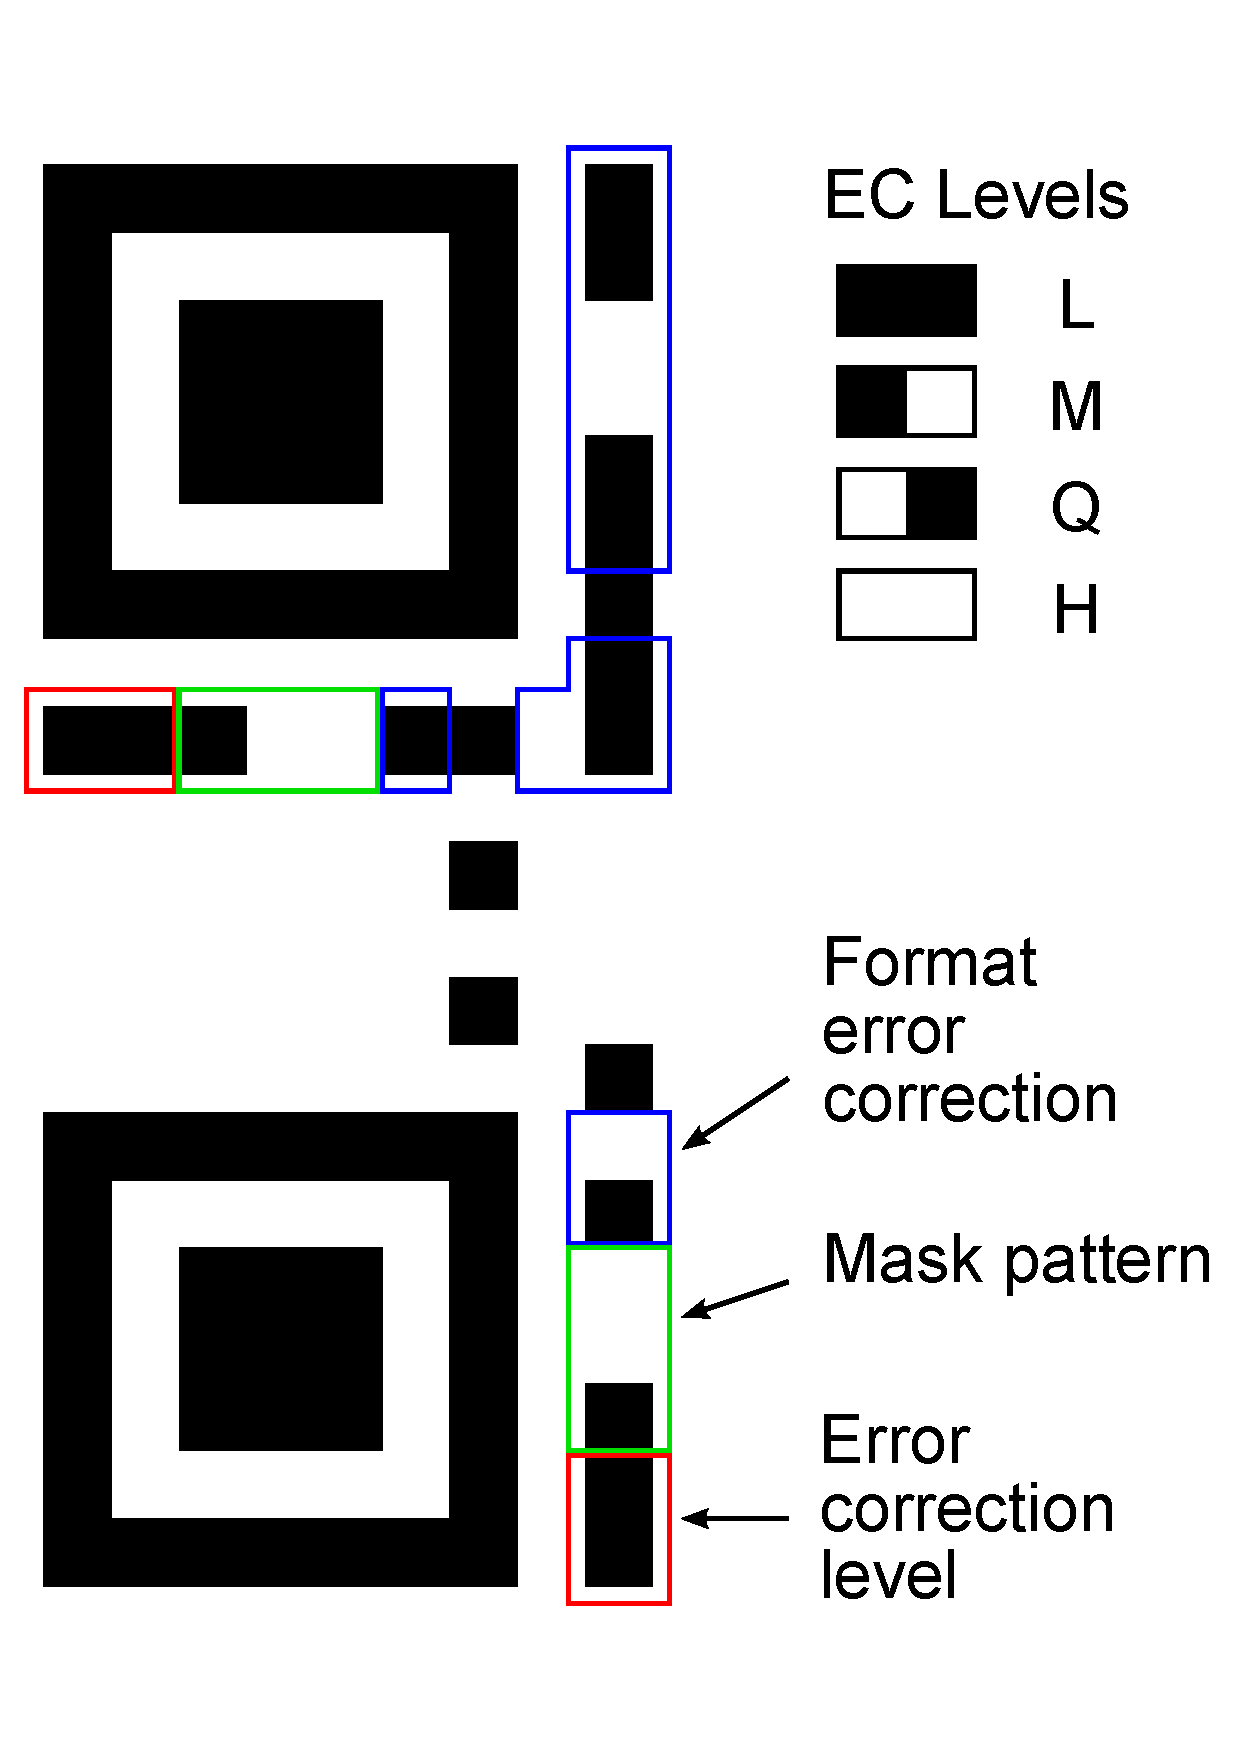
\includegraphics[height=0.4\textwidth]{figures/QR_Format_Information.pdf}
	\caption{Metadaten eines QR-Codes (Stufe L) \cite{QRCode2024}}
	\label{fig:qrschema}
\end{figure}
Die Nutzdaten sind wie in Abbildung \ref{fig:qrdata} als Symbole mit je acht Modulen codiert.
Es können insgesamt 26 Symbole im QR-Code platziert werden.
Bei dem eingesetzten Reed-Solomon-Code $RS(255,248)$ gekürzt auf $RS(26,19)$ sind 19 Symbole für die Nutzdaten und die sieben Symbole E1 bis E7 für die Fehlertoleranz.
Da aber zur Überprüfung nochmals zwei Symbole der Nachricht als Metadaten gebraucht werden, nur 17 Symbole für die eigentliche Nachricht \cite{pillazoHowDecodeQR2013}.
Damit können bis zu 2 Symbole also 16 Module korrigiert werden \cite{QRCode2024}.
\begin{figure}[ht]
	\centering
	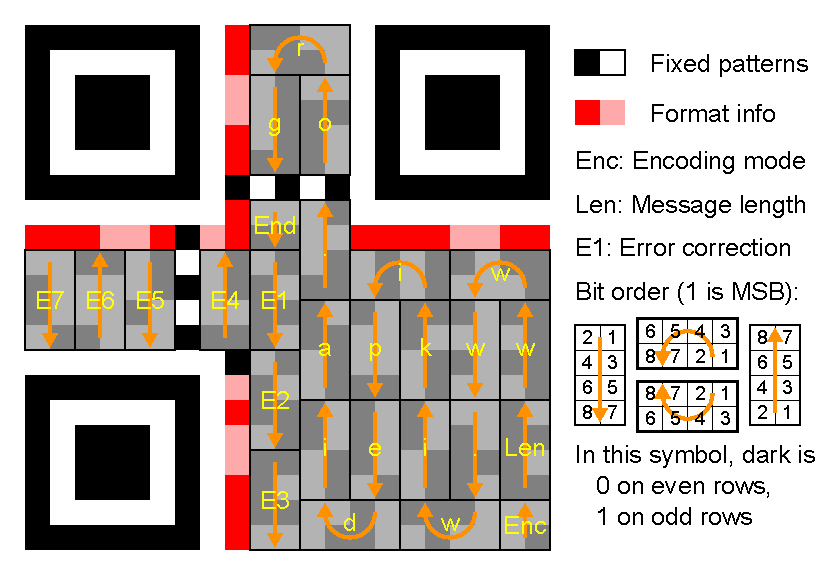
\includegraphics[height=0.4\textwidth]{figures/QR_Character_Placement.pdf}
	\caption{Datensymbole in einem QR-Code (Stufe L) \cite{QRCode2024}}
	\label{fig:qrdata}
\end{figure}

Diese Fehlerkorrekturmechanismen ermöglichen QR-Codes Robustheit gegenüber physischen Beschädigungen wie Rissen, Kratzern oder Verunreinigungen. Die Fähigkeit, selbst in solch herausfordernden Bedingungen die gespeicherten Daten korrekt wiederherzustellen, hat zur weitverbreiteten Nutzung von QR-Codes in verschiedenen Bereichen geführt, darunter Marketing, Logistik und Zugangskontrollen \cite{QRCode2024}.

\backmatter
\listoffigures
\cleardoublepage

\listoftables
\cleardoublepage

\renewcommand{\lstlistlistingname}{List of Listings}  % change for German thesis
\lstlistoflistings
\cleardoublepage

\printnoidxglossaries

\sloppy
\printbibliography

\end{document}
